\appendix{}

\chapter{Supplemental Material for Chapter \ref{chap:chapter 1}}

Additional supplemental material can be found in the published location at \url{https://doi.org/10.2337/db24-0497}. 

\begin{figure}[h]
    \centering
    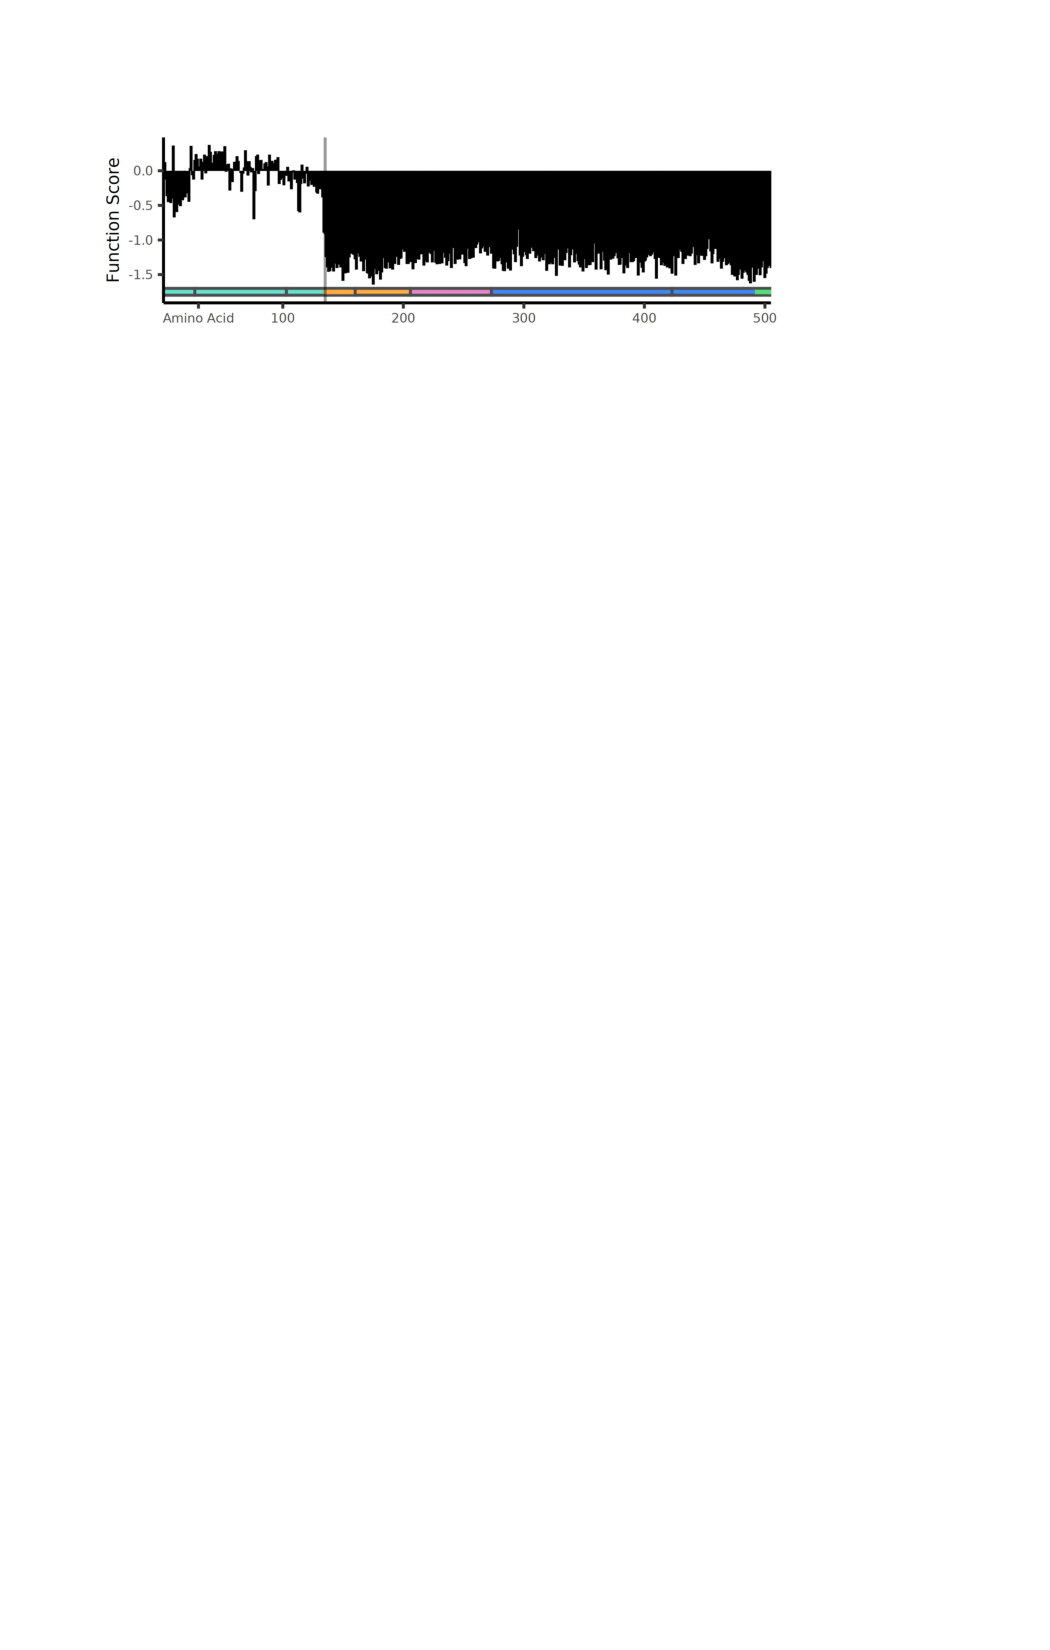
\includegraphics[width=\textwidth]{1_figures-and-files/FigS1.pdf}
    \caption[Alternative start site present with endogenous ligand.]{\textbf{Alternative start site present with endogenous ligand.} Function scores (FS) of insertions/deletions (indels) at each amino acid of PPAR$\gamma$2 calculated as previously published (Majithia et al. 2016) after 10 $\mu$M prostaglandin J2 (PGJ2) treatment. This response to an endogenous ligand is similar to the effect induced by the synthetic drug, rosiglitazone (\textbf{Figure 1.1D}). FS=0 refers to wild-type activity. 
    }
\end{figure}


\clearpage
\begin{table}[h]
  \centering
  \caption[CRISPR guides and genotypes from the monoclonal cell lines.]{\textbf{CRISPR guides and genotypes from the monoclonal cell lines.} Cell lines with guides targeted to \(PPARG\) intronic sequence (Int-sgRNA), to be used as control, targeted to exon 1 (Ex1-sgRNA), for pre-p.M135 edits, and targeted to exon 3 (Ex3-sgRNA), for post-p.M135 edits.
  }
\begin{tabular}{|c|c|c|m{4.7cm}|m{2.8cm}|}
    \hline
    Guide Name & Cut Site (hg38) & Zygosity & Genotype & Protein\newline Consequence \\
    \hline
    Int-sgRNA & chr3:12363492 & +/+ & WT & PPAR$\gamma$ \\
    \hline
    \multirow{4}{*}{Ex1-sgRNA} & \multirow{4}{*}{chr3:12379745} & \multirow{2}{*}{+/-} & chr3:12379749\_12379751delo\newline 12379744\_12379750del & p.N42GfsX50 \\
    \cline{4-5}
                                &                               &                       & chr3:12379736\_12379744delo\newline 12379741\_12379751del & p.T41SfsX48 \\
    \cline{3-5}
                                &                               & \multirow{2}{*}{-/-} & chr3:12379744\_12379973del & p.PPAR$\gamma\Delta$1 (deletion exon 1) \\
    \cline{4-5}
                               &                               &                       & chr3:12379702\_12379773del & p.PPAR$\gamma\Delta$1 (deletion exon 1) \\
    \cline{3-5}                                                        
    \hline
    \multirow{2}{*}{Ex3-sgRNA} & \multirow{2}{*}{chr3:12392733} & \multirow{2}{*}{-/-} & chr3:12392733insA & p.V201SfsX206 \\
    \cline{4-5}
                                &                               &                       & chr3:12392733insT & p.V201GfsX206 \\
    \hline
    \end{tabular}

\end{table}

\clearpage
\begin{figure}[h]
    \centering
    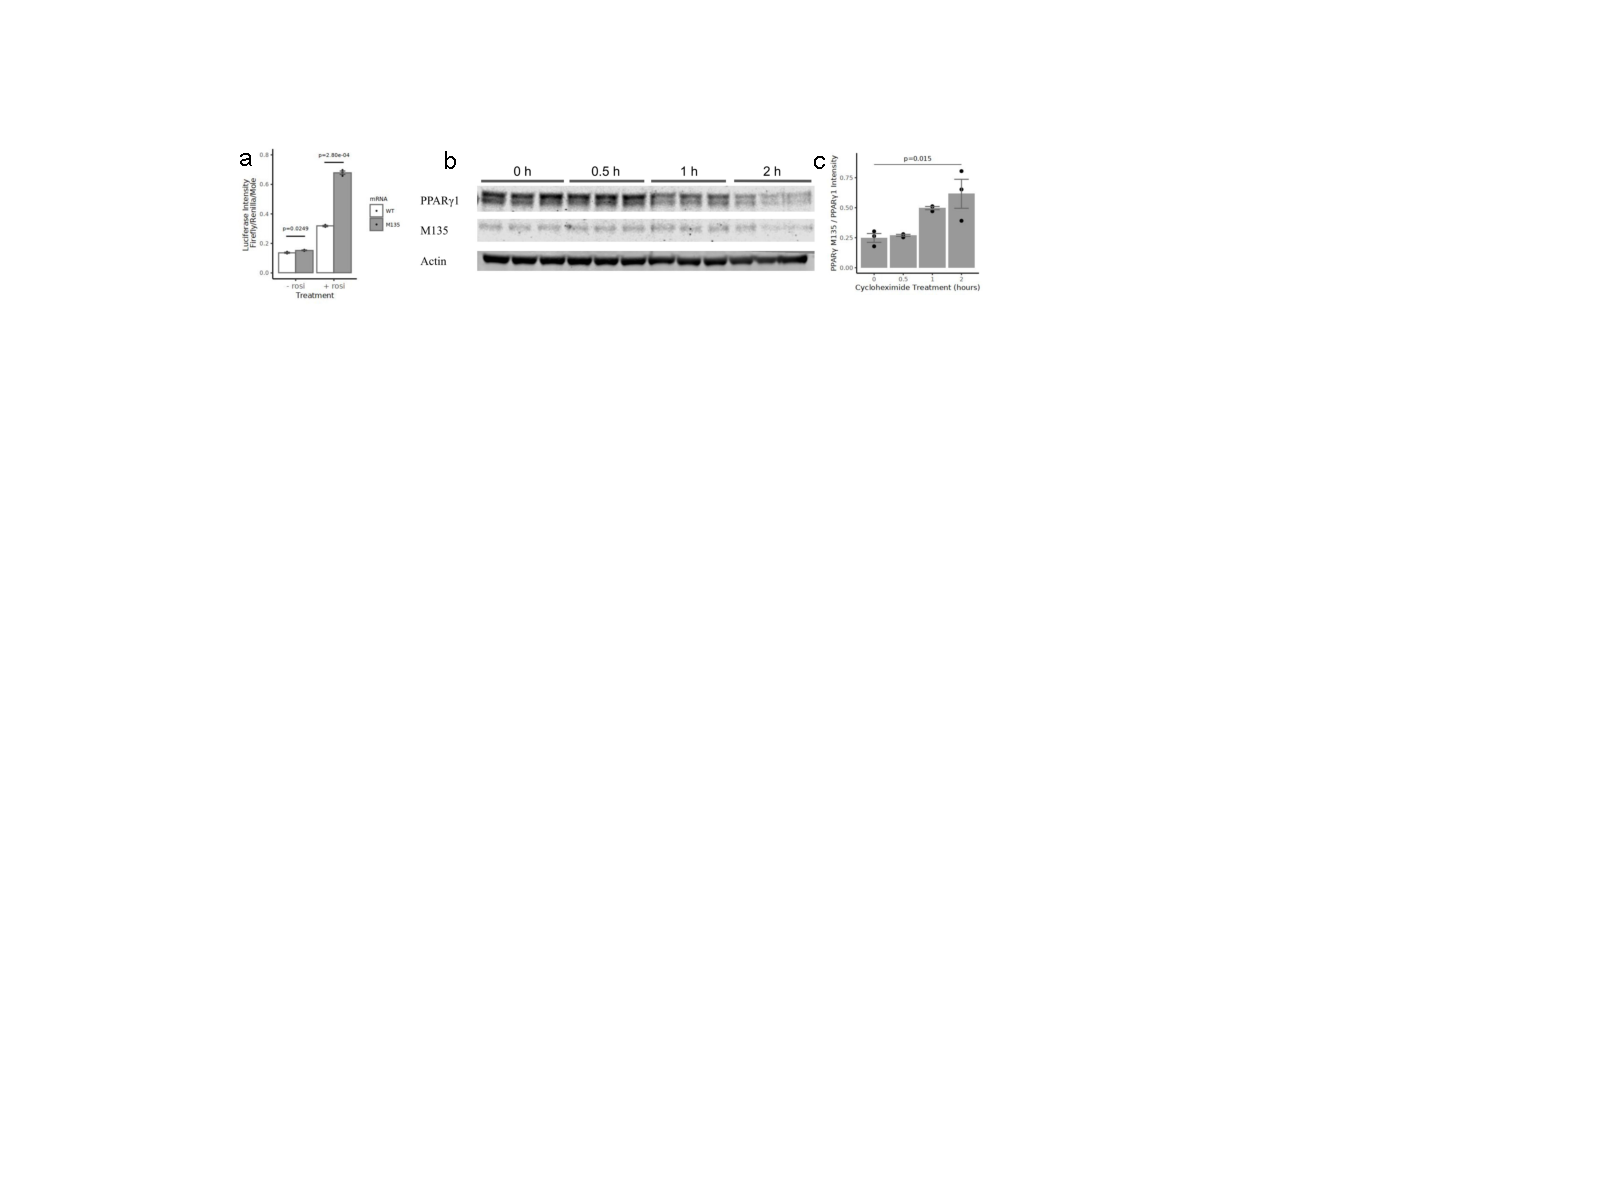
\includegraphics[width=\textwidth]{1_figures-and-files/FigS2.pdf}
    \caption[PPAR$\gamma$ M135 responds more strongly to ligands and degrades more slowly than PPAR$\gamma$1.]{\textbf{PPAR$\gamma$ M135 responds more strongly to ligands and degrades more slowly than PPAR$\gamma$1.} a. PPRE-driven luciferase promoter activity, normalized to Renilla and by mRNA moles, with 0 and 0.5 uM rosiglitazone treatments. PPAR$\gamma$ M135 activates transcription more strongly than WT PPAR$\gamma$ at baseline (n=3 each, t-test) and even more potently when stimulated with rosiglitazone (n=3 each, t-test). b. Western blot for the C-terminus of PPAR$\gamma$ in heterozygous Ex1-sgRNA THP-1 cells, which endogenously express both PPAR$\gamma$1 and PPAR$\gamma$ M135, after a 0-2 hour treatment with 5 uM cycloheximide (n=3). Actin serves as the loading control. c. Mean and sem of PPAR$\gamma$ M135/PPAR$\gamma$1 measured from b. PPAR$\gamma$ M135/PPAR$\gamma$1 increases over time after protein synthesis arrest, indicating slower degradation of PPAR$\gamma$ M135. ANOVA with Tukey post hoc test shows a significant difference between 0 and 2 hour time points.
    }
\end{figure}

\clearpage
\begin{figure}[h]
    \centering
    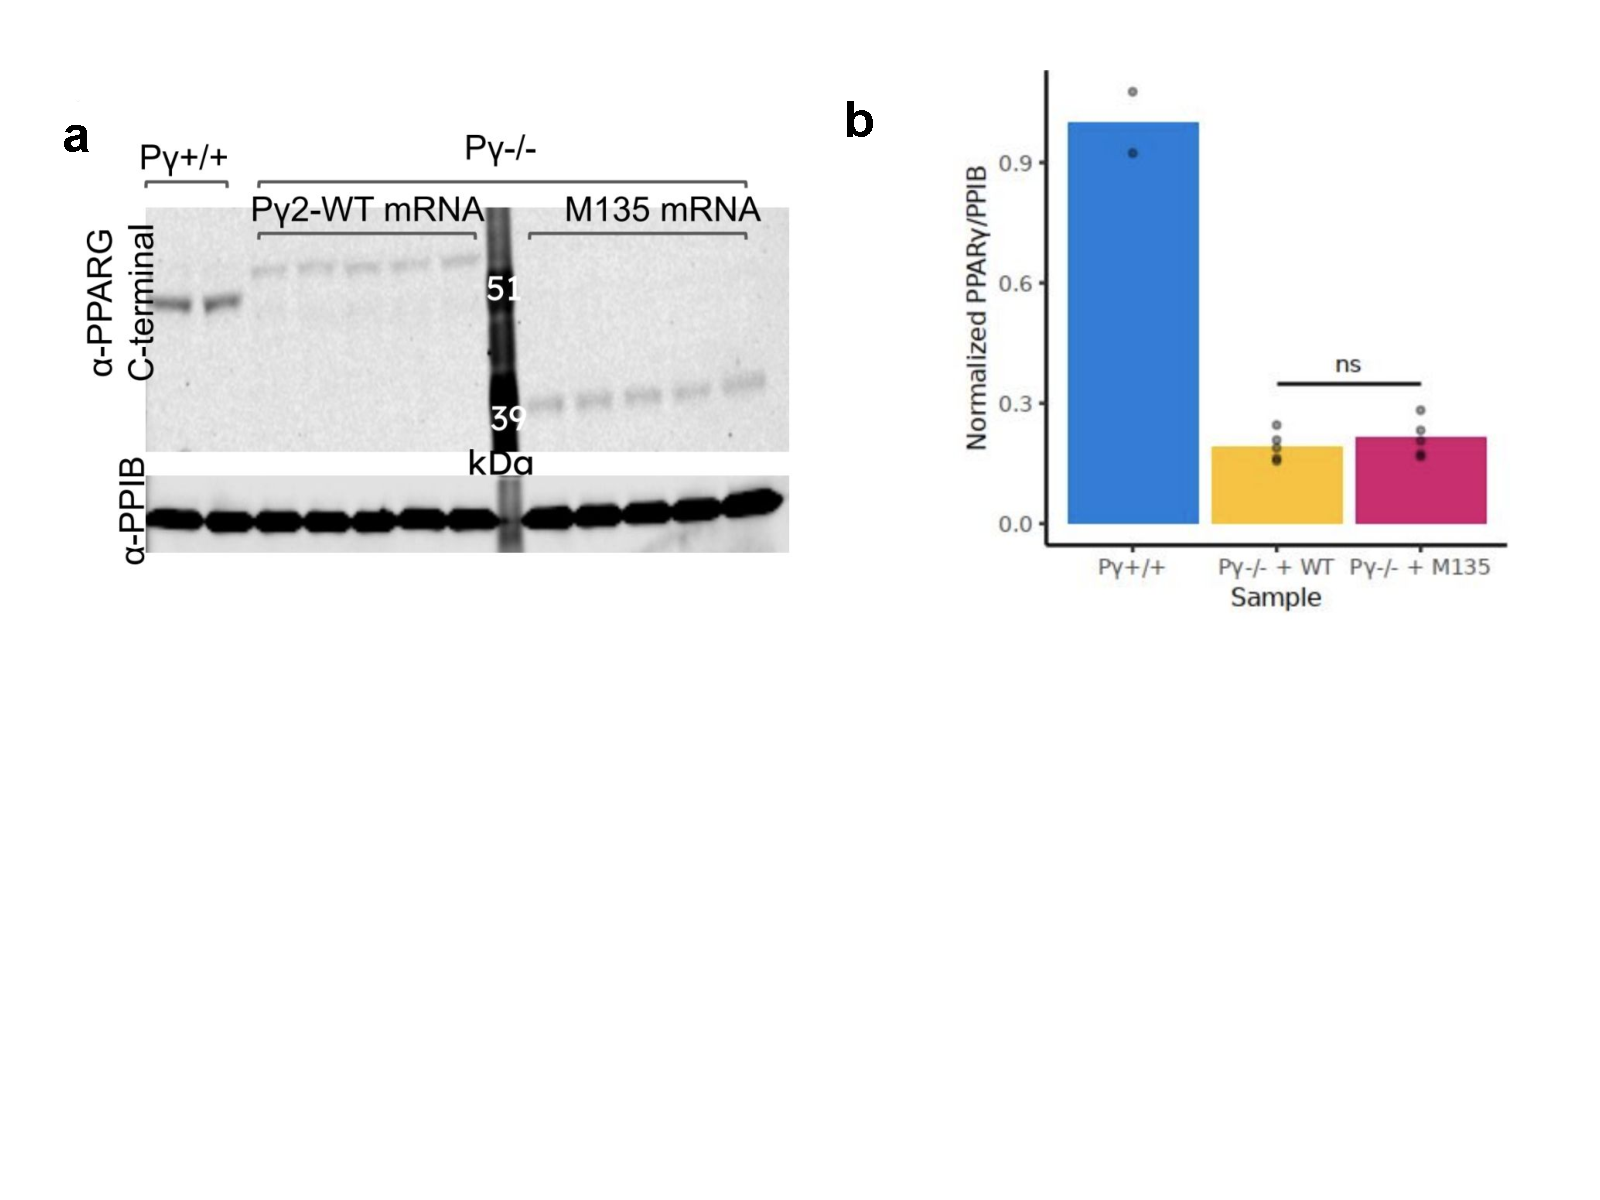
\includegraphics[width=\textwidth]{1_figures-and-files/FigS3.pdf}
    \caption[PPAR$\gamma$ protein abundance in rescue experiments.]{\textbf{PPAR$\gamma$ protein abundance in rescue experiments.} a. Western blot for the C-terminus of PPAR$\gamma$ with protein lysates from wild-type THP-1s (P$\gamma$+/+), PPAR$\gamma$ null THP-1s (P$\gamma$-/-) electroporated with PPAR$\gamma$2 wild-type (P$\gamma$2-WT) mRNA, and P$\gamma$-/- THP-1s electroporated with M135 mRNA. 8 $\mu$g WT mRNA and 2 $\mu$g M135 mRNA were electroporated to obtain similar protein expression. b. Normalized relative abundance of PPAR$\gamma$ protein in P$\gamma$+/+ (WT) THP-1, P$\gamma$-/- THP-1 electroporated with WT mRNA, and P$\gamma$-/- THP-1 electroporated with M135 mRNA. The ratio of PPAR$\gamma$ to the loading control of cyclophilin B (PPIB) was normalized to the mean of the P$\gamma$+/+ ratios, and data is presented as the mean with the data points. Statistical significance for the difference between P$\gamma$-/- + WT and P$\gamma$-/- + M135 was assessed by a two sample t-test, and the threshold used for significance was p=0.05.
    }
\end{figure}

\clearpage
\begin{table}[t]
    \centering
    \caption[Gene ontology pathway names for Figure 1.4.]{\textbf{Gene ontology pathway names for Figure 1.4.} GO IDs and pathways for the 28 pathways identified by the M135-specific DEGs.}
    \begin{tabular}{|c|m{13cm}|}
    \hline
        GO ID & GO Pathway Name \\ 
        \hline
        GO:0071674 & GOBP\_MONONUCLEAR\_CELL\_MIGRATION \\ 
        \hline
        GO:0009615 & GOBP\_RESPONSE\_TO\_VIRUS \\ \hline
        GO:0002252 & GOBP\_IMMUNE\_EFFECTOR\_PROCESS \\ \hline
        GO:0002684 & GOBP\_POSITIVE\_REGULATION\_OF\_IMMUNE\_SYSTEM\_PROCESS \\ \hline
        GO:0019079 & GOBP\_VIRAL\_GENOME\_REPLICATION \\ \hline
        GO:0006954 & GOBP\_INFLAMMATORY\_RESPONSE \\ \hline
        GO:0002711 & GOBP\_POSITIVE\_REGULATION\_OF\_T\_CELL\_MEDIATED\_IMMUNITY \\ \hline
        GO:0042330 & GOBP\_TAXIS \\ \hline
        GO:0002521 & GOBP\_LEUKOCYTE\_DIFFERENTIATION \\ \hline
        GO:0008284 & GOBP\_POSITIVE\_REGULATION\_OF\_CELL\_\newline POPULATION\_PROLIFERATION \\ \hline
        GO:0010628 & GOBP\_POSITIVE\_REGULATION\_OF\_GENE\_EXPRESSION \\ \hline
        GO:0003013 & GOBP\_CIRCULATORY\_SYSTEM\_PROCESS \\ \hline
        GO:0048878 & GOBP\_CHEMICAL\_HOMEOSTASIS \\ \hline
        GO:0051338 & GOBP\_REGULATION\_OF\_TRANSFERASE\_ACTIVITY \\ \hline
        GO:0051050 & GOBP\_POSITIVE\_REGULATION\_OF\_TRANSPORT \\ \hline
        GO:0048732 & GOBP\_GLAND\_DEVELOPMENT \\ \hline
        GO:0051301 & GOBP\_CELL\_DIVISION \\ \hline
        GO:0051130 & GOBP\_POSITIVE\_REGULATION\_OF\_CELLULAR\_\newline COMPONENT\_ORGANIZATION \\ \hline
        GO:1903047 & GOBP\_MITOTIC\_CELL\_CYCLE\_PROCESS \\ \hline
        GO:1901135 & GOBP\_CARBOHYDRATE\_DERIVATIVE\_METABOLIC\_PROCESS \\ \hline
        GO:0043254 & GOBP\_REGULATION\_OF\_PROTEIN\_CONTAINING\_\newline COMPLEX\_ASSEMBLY \\ \hline
        GO:0033865 & GOBP\_NUCLEOSIDE\_BISPHOSPHATE\_METABOLIC\_PROCESS \\ \hline
        GO:0046039 & GOBP\_GTP\_METABOLIC\_PROCESS \\ \hline
        GO:0043604 & GOBP\_AMIDE\_BIOSYNTHETIC\_PROCESS \\ \hline
        GO:0042274 & GOBP\_RIBOSOMAL\_SMALL\_SUBUNIT\_BIOGENESIS \\ \hline
        GO:0042255 & GOBP\_RIBOSOME\_ASSEMBLY \\ \hline
        GO:0042254 & GOBP\_RIBOSOME\_BIOGENESIS \\ \hline
        GO:0002181 & GOBP\_CYTOPLASMIC\_TRANSLATION \\ \hline
    \end{tabular}
\end{table}